% Provenance (never printed): old seconde/premiere S material on the ocean
% (the ocean as a layered fluid, its heat, upwelling and productive waters);
% see sources/book2/PROVENANCE.md. All profiles are WOA23 columns, all
% densities the EOS-80 one-atmosphere equation, computed in
% figdata/grade-10/ocean_profiles.py.
\chapter{De gelaagde oceaan}\label{ch:g10:layered-ocean}

Op een zomerdag zwem je vanaf een strand de zee in, in water dat aangenaam warm
is. Dan laat je je benen naar beneden hangen --- en je voeten voelen water dat
een paar meter onder het oppervlak opeens koud is. De zee is niet van boven tot
onder gemengd: ze bestaat uit lagen, warm en licht boven, koud en dicht onder.
In de open oceaan reikt diezelfde \omterm{def:g10:layered-ocean:stratification}{gelaagdheid} kilometers diep, en ze bepaalt waar
de zee een woestijn is en waar ze wemelt van het leven. Dit hoofdstuk bekijkt de
oceaan in de diepte: hoe hij wordt gemeten, hoe zijn temperatuur en zoutgehalte
naar beneden toe veranderen, waarom de lagen stabiel zijn, en waar koud diep
water weer naar het oppervlak komt.

\begin{recall}
Zeewater bevat opgeloste zouten: zijn zoutgehalte, gemiddeld ongeveer 35 gram
zout per kilogram zeewater, verschilt van zee tot zee. Winden drijven de
oppervlaktestromingen en de grote kringvormige gyres aan; diepe stromingen van
koud, zout water bewegen langzaam over de oceaanbodem (Boek 1, jaar 8).
Dichtheid is massa gedeeld door volume (de natuurkundeboeken). Het
fytoplankton, microscopisch kleine algen, heeft licht en minerale
voedingsstoffen nodig om door fotosynthese te groeien, en het voedt de rest van
de voedselketens van de oceaan (de biologieboeken).
\end{recall}

\section{De oceaan meten}

De oceaan bedekt ongeveer \num{362}~miljoen~\unit{km^2} en is gemiddeld
\qty{3682}{m} diep: zo'n \num{1.33}~miljard~\unit{km^3} water. Het grootste deel
ligt ver buiten het bereik van het licht, en kan alleen worden gemeten door er
instrumenten naartoe te laten zakken.
% ledger: charette:ocean-volume

Vanaf een schip laten oceanografen aan een kabel een frame zakken met sensoren
die de geleidbaarheid van het water meten (waaruit het zoutgehalte wordt
berekend), de temperatuur en de druk (en dus de diepte), omringd door een krans
van flessen die op gekozen diepten worden gesloten om watermonsters aan boord te
brengen. Sinds 2000 heeft een vloot van robotboeien er miljoenen profielen aan
toegevoegd: elke boei drijft met de stromingen mee op een diepte van
\qty{1000}{m}, zakt ongeveer elke tien dagen naar \qty{2000}{m}, stijgt dan naar
het oppervlak terwijl ze onderweg temperatuur en zoutgehalte meet, en verstuurt
haar profiel via een satelliet.
% ledger: argo:fleet

\begin{dated}{2026}
Het internationale Argo-netwerk telt bijna 4000 actieve boeien; het
drie miljoenste profiel werd in juli 2024 verzameld.
% ledger: argo:fleet
\end{dated}

\begin{omfigure}
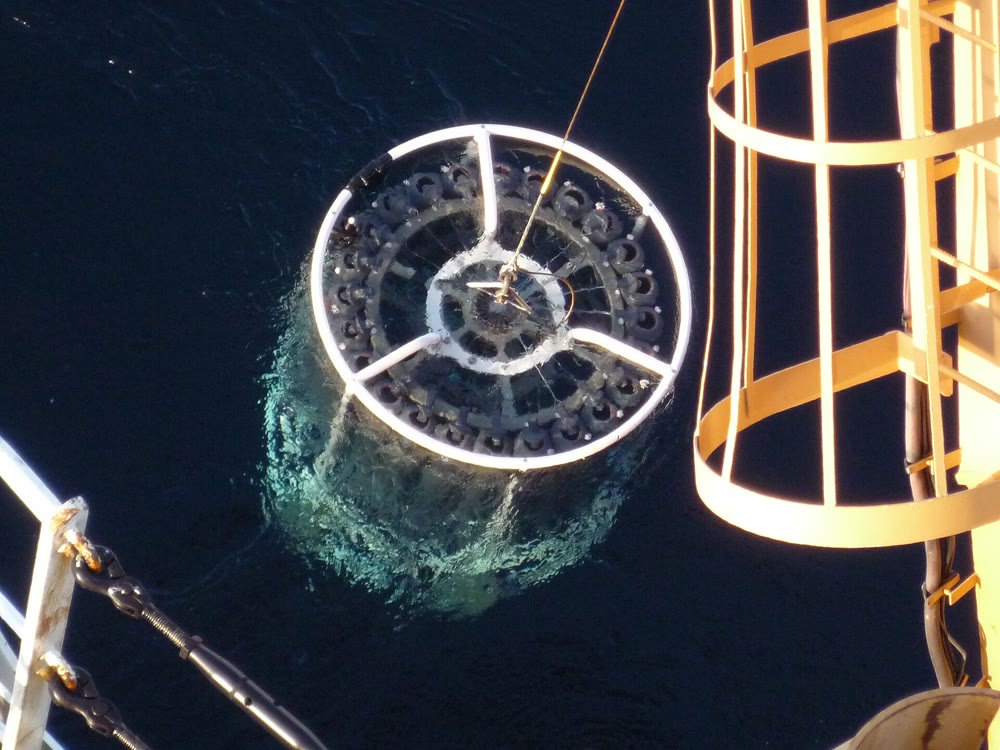
\includegraphics[height=4.4cm]{images/book2/g10-noaa-ctd-rosette.jpg}\hspace{0.4cm}%
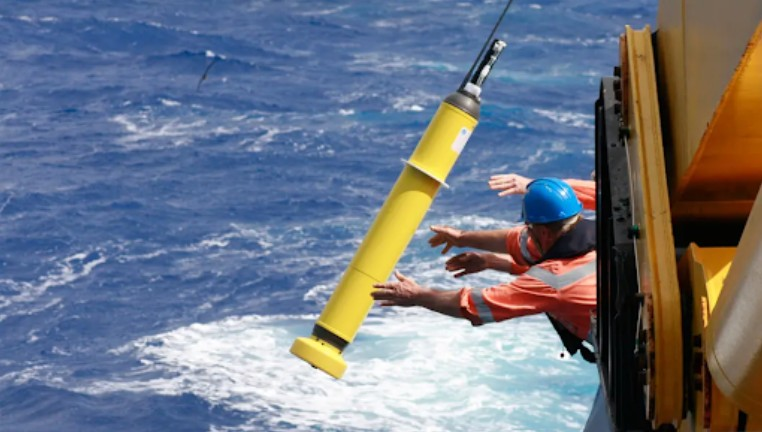
\includegraphics[height=4.4cm]{images/book2/g10-noaa-argo-float.jpg}

{\small Links: een rozet van monsterflessen rond de sensoren, naast een
onderzoeksschip in het Noordpoolgebied weer omhooggehaald, 2008 (foto: Pablo
Clemente-Colon, NOAA Photo Library). Rechts: een profielboei wordt vanaf een
onderzoeksschip te water gelaten (foto: NOAA Global Ocean Monitoring and
Observing Program). Beide publiek domein.}
\end{omfigure}

Gemiddeld over decennia van metingen geven deze profielen een beeld van de
oceaan in de diepte. De profielen van dit hoofdstuk zijn zulke gemiddelden, uit
de \emph{World Ocean Atlas 2023} van de NOAA National Centers for Environmental
Information.

\section{Temperatuur en diepte}

\begin{omfigure}
\begin{tikzpicture}
\begin{axis}[omrecord, omdepth, width=0.62\linewidth, height=8.2cm,
  axis x line=top, xmin=-3, xmax=31, ymin=0, ymax=2000,
  xlabel={temperatuur (\unit{\degreeCelsius})}, ylabel={diepte (\unit{m})},
  tick label style={font=\small}, label style={font=\small},
  legend style={font=\scriptsize, at={(0.98,0.03)}, anchor=south east}]
\addplot[omThm!85!black, thick] table[x=t, y=depth] {figdata/out/grade-10-ocean_profiles-site-warmpool.dat};
\addplot[omDef!85!black, thick] table[x=t, y=depth] {figdata/out/grade-10-ocean_profiles-site-atlantic.dat};
\addplot[black!70, thick, dashed] table[x=t, y=depth] {figdata/out/grade-10-ocean_profiles-site-arctic.dat};
\legend{{tropische Grote Oceaan, 5.5\textdegree NB}, {noordelijke Atlantische Oceaan, 40.5\textdegree NB}, {Noordelijke IJszee, 75.5\textdegree NB}}
\node[font=\scriptsize, anchor=west] (ml) at (axis cs:21,430) {gemengde laag};
\draw[black!50] (ml.north east) -- (axis cs:28.9,35);
\node[font=\scriptsize, anchor=west] (tc) at (axis cs:15.5,600) {thermocline};
\draw[black!50] (tc.north) -- (axis cs:19.9,150);
\node[font=\scriptsize, anchor=west] at (axis cs:7,1500) {diepe oceaan};
\end{axis}
\end{tikzpicture}

{\small Gemiddelde temperatuur tegen de diepte op drie plaatsen (de diepte neemt
naar beneden toe). Gegevens: World Ocean Atlas 2023, jaargemiddelden, NOAA NCEI.}
\end{omfigure}
% ledger: data:b2-woa23 (profiles in figdata/grade-10/ocean_profiles.py)

Zonlicht verwarmt de oceaan van boven, in zijn oppervlaktelaag. Wind en golven
mengen dit warme water tot een laag met een bijna uniforme temperatuur. Daaronder
daalt de temperatuur snel over een paar honderd meter; nog dieper daalt ze
langzaam tot het koude water dat de oceaanbekkens vult.

\begin{definition}[Gemengde laag]\label{def:g10:layered-ocean:mixed-layer}
De \emph{gemengde laag}\index{gemengde laag} is de oppervlaktelaag van de
oceaan, die door wind en golven wordt gemengd, waarin temperatuur en
zoutgehalte nauwelijks met de diepte veranderen.
\end{definition}

\begin{definition}[Thermocline; halocline; pycnocline; diepe oceaan]\label{def:g10:layered-ocean:thermocline}
De \emph{thermocline}\index{thermocline} is de laag onder de \omterm{def:g10:layered-ocean:mixed-layer}{gemengde laag}
waarin de temperatuur snel daalt met de diepte. De laag waarin het zoutgehalte
snel verandert met de diepte, is een \emph{halocline}\index{halocline}; de laag
waarin de dichtheid snel toeneemt met de diepte, is de
\emph{pycnocline}\index{pycnocline}. Daaronder ligt de \emph{diepe
oceaan}\index{diepe oceaan}, koud en langzaam veranderend.
\end{definition}

In de tropische Grote Oceaan is de \omterm{def:g10:layered-ocean:mixed-layer}{gemengde laag} \qty{29.2}{\degreeCelsius}
warm en zo'n \qty{60}{m} dik; tussen \qty{70}{m} en \qty{300}{m} daalt de
temperatuur met bijna negentien graden, en op \qty{1000}{m} is ze gezakt tot
\qty{4.5}{\degreeCelsius}. In de noordelijke Atlantische Oceaan is het oppervlak
koeler en de daling geleidelijker. In de Noordelijke IJszee blijft de hele kolom
binnen twee graden van \qty{0}{\degreeCelsius}: van een warme oppervlaktelaag
is nauwelijks sprake.
% ledger: data:b2-woa23

\begin{method}[Een oceaanprofiel lezen]\label{met:g10:layered-ocean:profile}
\begin{enumerate}
  \item Zoek de assen: de diepte neemt naar beneden toe, de gemeten grootheid
        lees je langs de bovenkant af.
  \item De \omterm{def:g10:layered-ocean:mixed-layer}{gemengde laag} is het bovenste deel, waar de kromme bijna verticaal
        loopt; haar diepte is de plaats waar de kromme begint af te buigen (een
        gangbare regel: waar de temperatuur \qty{0.5}{\degreeCelsius} onder haar
        waarde aan het oppervlak is gedaald).
  \item De \omterm{def:g10:layered-ocean:thermocline}{thermocline} is waar de kromme het dichtst bij horizontaal ligt: de
        grootste verandering over de kleinste diepte.
  \item Lees daaronder de diepe waarden af, en vergelijk plaatsen op dezelfde diepte.
\end{enumerate}
\end{method}

De \omterm{def:g10:layered-ocean:mixed-layer}{gemengde laag} verandert met de seizoenen. In de winter verliest het oppervlak
warmte, stormen woelen de zee om en de \omterm{def:g10:layered-ocean:mixed-layer}{gemengde laag} wordt dieper; in de zomer
verwarmt de zon een dunne oppervlaktelaag die de zachtere winden niet naar
beneden kunnen mengen, en ontstaat er dicht bij het oppervlak een
\emph{seizoensthermocline} --- het koude water dat de voeten van de zwemmer voelen.

\begin{omfigure}
\begin{tikzpicture}
\begin{axis}[omrecord, omdepth, width=0.6\linewidth, height=6.6cm,
  axis x line=top, xmin=12, xmax=24, ymin=0, ymax=300,
  xlabel={temperatuur (\unit{\degreeCelsius})}, ylabel={diepte (\unit{m})},
  tick label style={font=\small}, label style={font=\small},
  legend style={font=\scriptsize, at={(0.98,0.03)}, anchor=south east}]
\addplot[omDef!85!black, thick] table[x=t_feb, y=depth] {figdata/out/grade-10-ocean_profiles-season.dat};
\addplot[omThm!85!black, thick] table[x=t_aug, y=depth] {figdata/out/grade-10-ocean_profiles-season.dat};
\legend{februari, augustus}
\end{axis}
\end{tikzpicture}

{\small Winter en zomer in de noordelijke Atlantische Oceaan (40.5\textdegree NB,
30.5\textdegree WL): maandgemiddelde temperaturen voor februari en augustus.
In februari reikt de \omterm{def:g10:layered-ocean:mixed-layer}{gemengde laag} tot ongeveer \qty{170}{m}; in augustus ligt
een warme laag van ongeveer \qty{15}{m} dik op een seizoensthermocline.
Gegevens: World Ocean Atlas 2023, NOAA NCEI.}
\end{omfigure}
% ledger: data:b2-woa23 (mixed-layer depths by the 0.5 degC rule, computed in figdata/grade-10/ocean_profiles.py)

\section{Zoutgehalte en dichtheid}

De dichtheid van zeewater hangt af van zijn temperatuur en zijn zoutgehalte. Ze
wordt berekend met een internationaal afgesproken formule, de toestandsvergelijking
van zeewater, die op laboratoriummetingen is aangepast.

\begin{proposition}[Dichtheid van zeewater]\label{prop:g10:layered-ocean:density}
De dichtheid van zeewater neemt toe met zijn zoutgehalte en af naarmate zijn
temperatuur stijgt. Bij de druk aan het oppervlak heeft zeewater met zoutgehalte
35 een dichtheid van \qty{1028.1}{kg/m^3} bij \qty{0}{\degreeCelsius} en
\qty{1023.3}{kg/m^3} bij \qty{25}{\degreeCelsius}; zuiver water van
\qty{4}{\degreeCelsius} heeft een dichtheid van \qty{1000.0}{kg/m^3}.
\end{proposition}
% ledger: unesco:eos80 (values computed in figdata/grade-10/ocean_profiles.py)

\begin{omfigure}
\begin{tikzpicture}
\begin{axis}[omrecord, width=0.7\linewidth, height=6.2cm, xmin=-2, xmax=30,
  ymin=1016, ymax=1033, xlabel={temperatuur (\unit{\degreeCelsius})},
  ylabel={dichtheid (\unit{kg/m^3})}, tick label style={font=\small},
  label style={font=\small}, yticklabel style={/pgf/number format/1000 sep={}}]
\addplot[omThm!85!black, thick] table[x=t, y=rho_s38] {figdata/out/grade-10-ocean_profiles-eos.dat};
\addplot[black!80, thick] table[x=t, y=rho_s35] {figdata/out/grade-10-ocean_profiles-eos.dat};
\addplot[omDef!85!black, thick] table[x=t, y=rho_s30] {figdata/out/grade-10-ocean_profiles-eos.dat};
\node[font=\scriptsize, anchor=south west, omThm!85!black] at (axis cs:1,1030.75) {zoutgehalte 38};
\node[font=\scriptsize, anchor=south west] at (axis cs:1,1028.35) {zoutgehalte 35};
\node[font=\scriptsize, anchor=south west, omDef!85!black] at (axis cs:1,1024.35) {zoutgehalte 30};
\end{axis}
\end{tikzpicture}

{\small De dichtheid van zeewater bij de druk aan het oppervlak, tegen zijn
temperatuur, voor drie zoutgehalten (berekend met de internationale
toestandsvergelijking van zeewater).}
\end{omfigure}
% ledger: unesco:eos80

De grafiek laat twee dingen zien. Eén eenheid zoutgehalte voegt ongeveer
\qty{0.8}{kg/m^3} toe. Eén graad opwarming haalt er ongeveer \qty{0.31}{kg/m^3}
af bij \qty{25}{\degreeCelsius}, \qty{0.18}{kg/m^3} bij \qty{10}{\degreeCelsius},
maar slechts \qty{0.06}{kg/m^3} rond \qty{0}{\degreeCelsius}: in warme zeeën
bepaalt de temperatuur de dichtheid, in koude zeeën het zoutgehalte.
% ledger: unesco:eos80 (slopes computed in figdata/grade-10/ocean_profiles.py)

\begin{remark}
De dichtheden van dit hoofdstuk zijn berekend bij de druk aan het oppervlak. De
druk van het water erboven drukt zeewater een beetje samen, met ongeveer
\qty{4}{kg/m^3} per kilometer diepte; oceanografen vergelijken watermassa's bij
dezelfde druk, zodat alleen temperatuur en zoutgehalte meetellen.
\end{remark}
% ledger: unesco:eos80-checks (computed in figdata/grade-10/ocean_profiles.py: 3.9 kg/m3 per km from the 10000-dbar check values)

\begin{omfigure}
\begin{tikzpicture}
\begin{axis}[name=sal, omrecord, omdepth, width=0.5\linewidth, height=7.2cm,
  axis x line=top, xmin=27.5, xmax=37, ymin=0, ymax=1000,
  xlabel={zoutgehalte}, ylabel={diepte (\unit{m})},
  tick label style={font=\small}, label style={font=\small}]
\addplot[omThm!85!black, thick] table[x=s, y=depth] {figdata/out/grade-10-ocean_profiles-site-warmpool.dat};
\addplot[omDef!85!black, thick] table[x=s, y=depth] {figdata/out/grade-10-ocean_profiles-site-atlantic.dat};
\addplot[black!70, thick, dashed] table[x=s, y=depth] {figdata/out/grade-10-ocean_profiles-site-arctic.dat};
\node[font=\scriptsize, anchor=west, align=left] at (axis cs:28.2,120) {arctische\\halocline};
\end{axis}
\begin{axis}[at={(sal.east)}, anchor=west, xshift=0.9cm, omrecord, omdepth,
  width=0.5\linewidth, height=7.2cm, axis x line=top, xmin=1021, xmax=1028.5, yticklabels={},
  ymin=0, ymax=1000, xlabel={dichtheid (\unit{kg/m^3})},
  tick label style={font=\small}, label style={font=\small},
  xticklabel style={/pgf/number format/1000 sep={}},
  legend style={font=\scriptsize, at={(0.03,0.03)}, anchor=south west}]
\addplot[omThm!85!black, thick] table[x=rho, y=depth] {figdata/out/grade-10-ocean_profiles-site-warmpool.dat};
\addplot[omDef!85!black, thick] table[x=rho, y=depth] {figdata/out/grade-10-ocean_profiles-site-atlantic.dat};
\addplot[black!70, thick, dashed] table[x=rho, y=depth] {figdata/out/grade-10-ocean_profiles-site-arctic.dat};
\legend{tropische Grote Oceaan, noordelijke Atlantische Oceaan, Noordelijke IJszee}
\end{axis}
\end{tikzpicture}

{\small Zoutgehalte (links) en dichtheid bij de druk aan het oppervlak (rechts)
tegen de diepte, op de drie plaatsen van de temperatuurprofielen. Op elke plaats
neemt de dichtheid naar beneden toe. Gegevens: World Ocean Atlas 2023, NOAA NCEI;
dichtheden uit de internationale toestandsvergelijking van zeewater.}
\end{omfigure}
% ledger: data:b2-woa23, unesco:eos80

In de tropische Grote Oceaan valt de \omterm{def:g10:layered-ocean:thermocline}{pycnocline} samen met de \omterm{def:g10:layered-ocean:thermocline}{thermocline}. In de
Noordelijke IJszee verandert de temperatuur nauwelijks, maar het zoutgehalte
stijgt van 28 aan het oppervlak, verzoet door rivieren en smeltend ijs, tot 34.8
op \qty{500}{m}: de \omterm{def:g10:layered-ocean:thermocline}{halocline} is de \omterm{def:g10:layered-ocean:thermocline}{pycnocline}. In elk geval neemt de dichtheid
naar beneden toe.
% ledger: data:b2-woa23

\begin{definition}[Gelaagdheid]\label{def:g10:layered-ocean:stratification}
De oceaan is \emph{gelaagd}\index{gelaagdheid} wanneer zijn dichtheid toeneemt
met de diepte: lichter water ligt in lagen op dichter water.
\end{definition}

Een gelaagde oceaan is stabiel. Een waterpakketje dat naar beneden in dichter
water wordt geduwd, is lichter dan zijn omgeving en drijft weer omhoog; een
pakketje dat omhoog wordt geduwd, zakt terug. Om de lagen te mengen moet de wind
hiertegen in werken, en hoe sterker de \omterm{def:g10:layered-ocean:thermocline}{pycnocline}, hoe moeilijker dat is: de
\omterm{def:g10:layered-ocean:thermocline}{thermocline} is een deksel dat het oppervlak van de \omterm{def:g10:layered-ocean:thermocline}{diepe oceaan} scheidt. De \omterm{def:g10:layered-ocean:thermocline}{diepe
oceaan} is gevuld met water dat lang geleden is gezonken in de koude poolzeeën,
waar oppervlaktewater dicht genoeg wordt om te zinken (Boek 1, jaar 8).

\section{Opwelling}

\begin{definition}[Opwelling]\label{def:g10:layered-ocean:upwelling}
\emph{Opwelling}\index{opwelling} is het opstijgen van koud water van onder de
oppervlaktelaag, ter vervanging van oppervlaktewater dat door de wind wordt
weggeduwd. Ze komt voor langs sommige kusten en in de open oceaan.
\end{definition}
% ledger: noaa:upwelling

Langs een kust sleept de wind die evenwijdig aan de kust waait het
oppervlaktewater mee; door de draaiing van de Aarde volgt het water de wind niet
gewoon, maar buigt het ervan af, naar rechts op het noordelijk halfrond en naar
links op het zuidelijk halfrond (hoe dat werkt, komt aan bod in de universitaire
boeken). Voor de kust van Peru waait de wind langs de kust naar de evenaar, en
wordt het oppervlaktewater naar open zee geduwd; dicht bij de kust stijgt koud
water op om zijn plaats in te nemen. \omterm{def:g10:layered-ocean:upwelling}{Opwelling} vindt ook plaats langs de
evenaar, waar de passaatwinden het oppervlaktewater aan beide kanten wegduwen.
% ledger: noaa:upwelling, kessler:peru-upwelling

\begin{omfigure}
\begin{tikzpicture}[font=\footnotesize, >={Stealth[length=2mm]}]
  % ocean and thermocline
  \fill[omDef!12] (0,-3.2) rectangle (8.2,0);
  \fill[omDef!30] (0,-3.2) -- (0,-2.0) .. controls (3,-2.0) and (5.5,-1.6) .. (7.4,-0.35) -- (8.2,0) -- (8.2,-3.2) -- cycle;
  \draw[omDef!80!black, dashed] (0,-2.0) .. controls (3,-2.0) and (5.5,-1.6) .. (7.4,-0.35);
  \node[anchor=north west, omDef!80!black] at (0.1,-2.05) {thermocline};
  \node[anchor=west, black!70] at (0.15,-0.9) {warm oppervlaktewater};
  \node[anchor=west, black!70] at (0.15,-2.75) {koud water, rijk aan voedingsstoffen};
  % land
  \fill[omExo!30, draw=black!60] (7.0,-3.2) -- (8.2,-0.1) -- (8.6,0.0) -- (9.6,1.2) -- (10.6,2.2) -- (10.6,-3.2) -- cycle;
  \node[anchor=south, align=center] at (9.9,-1.6) {land};
  % surface flow and rising water
  \draw[->, thick, omThm!80!black] (7.2,-0.3) -- (3.6,-0.3);
  \node[anchor=south, omThm!80!black] at (5.4,-0.25) {oppervlaktewater naar zee geduwd};
  \foreach \x/\y in {6.1/-2.1, 6.8/-1.7} \draw[->, thick, omDef!80!black] (\x,\y) -- (\x+0.45,\y+1.15);
  \node[anchor=north, omDef!80!black, align=center] at (6.0,-2.25) {koud water stijgt op};
  % wind along the shore, northward: with west on the left and east on the
  % right the reader looks north, so the wind goes into the page
  \draw[black!70, thick] (2.6,1.0) circle (0.22);
  \draw[black!70, thick] (2.6,1.0) ++(45:0.22) -- ++(225:0.44) (2.6,1.0) ++(135:0.22) -- ++(315:0.44);
  \node[anchor=west, align=left] at (2.9,1.0) {wind langs de kust, naar de evenaar\\(naar het noorden, het blad in)};
  \node[anchor=north west, black!60] at (0,-3.25) {$\leftarrow$ west};
  \node[anchor=north east, black!60] at (10.6,-3.25) {oost $\rightarrow$};
\end{tikzpicture}

{\small \omterm{def:g10:layered-ocean:upwelling}{Opwelling} aan de kust van Peru (schematische doorsnede van west naar
oost, niet op schaal): de wind waait langs de kust naar de evenaar, naar het
noorden, het blad in; het oppervlaktewater buigt naar links af en wordt naar zee
geduwd; koud water van onder de \omterm{def:g10:layered-ocean:thermocline}{thermocline} stijgt dicht bij de kust op om het te vervangen.}
\end{omfigure}

Het water dat opstijgt, is niet alleen koud. Onder de verlichte oppervlaktelaag
laten de resten van dood plankton, die zinken en vergaan, de minerale
voedingsstoffen vrij die het fytoplankton nodig heeft. Terug in het licht maken
die voedingsstoffen de opwellingsgebieden tot de productiefste wateren van de
oceaan, met de rijkste visgronden. Waar de oceaan sterk \omterm{def:g10:layered-ocean:stratification}{gelaagd} is en niets diep
water omhoogbrengt, raakt de verlichte laag zonder voedingsstoffen: de centra
van de subtropische gyres zijn de woestijnen van de oceaan.
% ledger: noaa:upwelling

\begin{omfigure}
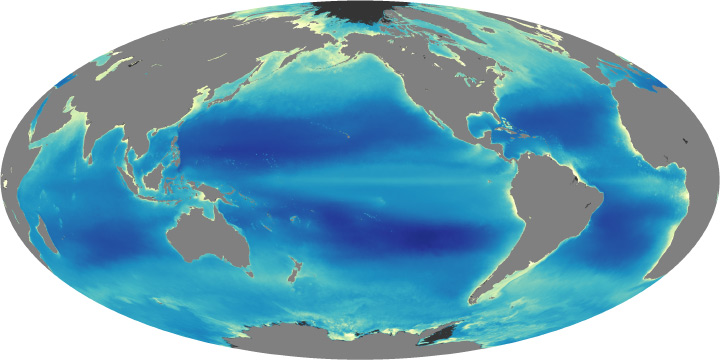
\includegraphics[width=0.8\linewidth]{images/book2/g10-nasa-ocean-chlorophyll.jpg}

{\small Het chlorofyl van het fytoplankton vanuit de ruimte gezien, gemiddeld
over 2002--2010: van donkerblauw (heel weinig) via lichtblauw tot geel (veel);
land in grijs. De kust van Peru en de band langs de evenaar in de Grote Oceaan
springen eruit; de gyres zijn diepblauw. Beeld: Jesse Allen en Robert Simmon,
NASA Earth Observatory (publiek domein).}
\end{omfigure}

\begin{omfigure}
\begin{tikzpicture}
\begin{axis}[omrecord, omdepth, width=0.6\linewidth, height=7.2cm,
  axis x line=top, xmin=4, xmax=26, ymin=0, ymax=600,
  xlabel={temperatuur (\unit{\degreeCelsius})}, ylabel={diepte (\unit{m})},
  tick label style={font=\small}, label style={font=\small},
  legend style={font=\scriptsize, at={(0.98,0.03)}, anchor=south east}]
\addplot[omExo!85!black, thick] table[x=t, y=depth] {figdata/out/grade-10-ocean_profiles-site-peru.dat};
\addplot[omThm!85!black, thick] table[x=t, y=depth] {figdata/out/grade-10-ocean_profiles-site-gyre.dat};
\addplot[black!40, dashed, domain=0:600, samples=2] ({15}, {x});
\legend{{voor Peru, 13.5\textdegree ZB}, {gyre van de zuidelijke Grote Oceaan, 20.5\textdegree ZB}}
\end{axis}
\end{tikzpicture}

{\small Voor de kust van Peru komt het koude water dicht bij het oppervlak: water
van \qty{15}{\degreeCelsius} (stippellijn) ligt op ongeveer \qty{65}{m}, tegen
bijna \qty{300}{m} midden in de gyre van de zuidelijke Grote Oceaan, die verder
van de evenaar ligt. Gegevens: World Ocean Atlas 2023, jaargemiddelden,
NOAA NCEI.}
\end{omfigure}
% ledger: data:b2-woa23

\section{Oefeningen}

\begin{exercise}[$\star$]\label{exo:g10:layered-ocean:1}
Definieer de \omterm{def:g10:layered-ocean:mixed-layer}{gemengde laag} en de \omterm{def:g10:layered-ocean:thermocline}{thermocline}. Wat mengt de \omterm{def:g10:layered-ocean:mixed-layer}{gemengde laag}?
\end{exercise}

\begin{exercise}[$\star$]\label{exo:g10:layered-ocean:2}
Definieer \omterm{def:g10:layered-ocean:upwelling}{opwelling}. Waarom zijn de wateren van opwellingsgebieden rijk aan leven?
\end{exercise}

\begin{exercise}[$\star$]\label{exo:g10:layered-ocean:3}
Geef met de temperatuurprofielen van de drie plaatsen de temperatuur aan het
oppervlak en op \qty{1000}{m} in de tropische Grote Oceaan en in de Noordelijke
IJszee.
\end{exercise}

\begin{exercise}[$\star$]\label{exo:g10:layered-ocean:4}
Wat is dichter: zeewater met zoutgehalte 35 bij \qty{25}{\degreeCelsius} of bij
\qty{0}{\degreeCelsius}? Zeewater met zoutgehalte 35 of zuiver water, bij
dezelfde temperatuur? Gebruik de waarden uit het hoofdstuk.
\end{exercise}

\begin{exercise}[$\star$]\label{exo:g10:layered-ocean:5}
Leg uit hoe een profielboei een profiel van de oceaan meet, en waarom boeien
nuttig zijn waar zelden schepen komen.
\end{exercise}

\begin{exercise}[$\star\star$]\label{exo:g10:layered-ocean:6}
De oceaan bedekt \num{361.84}~miljoen~\unit{km^2} met een gemiddelde diepte van
\qty{3682}{m}. Bereken zijn volume in kubieke kilometer. Welk deel van zijn
diepte vormen de bovenste \qty{100}{m}?
\end{exercise}

\begin{exercise}[$\star\star$]\label{exo:g10:layered-ocean:7}
In het augustusprofiel van de noordelijke Atlantische Oceaan is de temperatuur
\qty{22.7}{\degreeCelsius} aan het oppervlak, \qty{22.2}{\degreeCelsius} op
\qty{15}{m}, \qty{21.8}{\degreeCelsius} op \qty{20}{m} en
\qty{17.3}{\degreeCelsius} op \qty{50}{m}. Schat met de regel van de methode de
diepte van de \omterm{def:g10:layered-ocean:mixed-layer}{gemengde laag}. Hoe snel daalt de temperatuur gemiddeld tussen
\qty{20}{m} en \qty{50}{m}, in graden per meter?
\end{exercise}

\begin{exercise}[$\star\star$]\label{exo:g10:layered-ocean:8}
Op dezelfde plaats in de noordelijke Atlantische Oceaan is het oppervlak
\qty{15.3}{\degreeCelsius} in februari en \qty{22.7}{\degreeCelsius} in
augustus, terwijl het water op \qty{300}{m} in beide maanden
\qty{13.5}{\degreeCelsius} is. Leg uit waarom het diepe water de seizoenen niet
volgt, en waarom de \omterm{def:g10:layered-ocean:mixed-layer}{gemengde laag} in de winter veel dieper is dan in de zomer.
\end{exercise}

\begin{exercise}[$\star\star$]\label{exo:g10:layered-ocean:9}
Rond \qty{10}{\degreeCelsius} voegt één eenheid zoutgehalte
\qty{0.78}{kg/m^3} toe aan de dichtheid en haalt één graad opwarming er
\qty{0.18}{kg/m^3} af. Hoeveel graden opwarming heffen één eenheid zoutgehalte
op? Beantwoord dezelfde vraag rond \qty{0}{\degreeCelsius}, waar één graad er
maar \qty{0.06}{kg/m^3} af haalt. Wat besluit je voor de
poolzeeën?
\end{exercise}

\begin{exercise}[$\star\star$]\label{exo:g10:layered-ocean:10}
In de Noordelijke IJszee is het water aan het oppervlak \qty{-1.4}{\degreeCelsius}
met een zoutgehalte van 28.1, en op \qty{200}{m} \qty{-1.4}{\degreeCelsius}
met een zoutgehalte van 33.3. Hun dichtheden zijn \qty{1022.6}{kg/m^3} en
\qty{1026.8}{kg/m^3}. Wat maakt het diepere water dichter? Geef de naam van de
laag ertussen.
\end{exercise}

\begin{exercise}[$\star\star$]\label{exo:g10:layered-ocean:11}
Leg met een pakketje oppervlaktewater dat door een golf naar beneden wordt
geduwd uit waarom een gelaagde oceaan stabiel is.
\end{exercise}

\begin{exercise}[$\star\star\star$]\label{exo:g10:layered-ocean:12}
Een liter zeewater met zoutgehalte 35 van \qty{0}{\degreeCelsius} wordt
verwarmd tot \qty{25}{\degreeCelsius}. Bereken met de dichtheden uit het
hoofdstuk zijn massa, en dan zijn nieuwe volume. Hoeveel is het uitgezet, in
milliliter? Een oceaanlaag van \qty{700}{m} dik warmt in dezelfde verhouding op:
hoeveel wordt ze dikker? (Dit is een sterke overdrijving van de echte
opwarming van de oceaan, hier alleen gebruikt om het effect te laten zien.)
\end{exercise}

\begin{exercise}[$\star\star\star$]\label{exo:g10:layered-ocean:13}
In de tropische Grote Oceaan is de dichtheid \qty{1021.6}{kg/m^3} op \qty{50}{m}
en \qty{1026.0}{kg/m^3} op \qty{200}{m}; in de noordelijke Atlantische Oceaan
verandert de temperatuur in februari nauwelijks over de bovenste \qty{150}{m}.
In welke van de twee zou een storm het water gemakkelijker tot \qty{150}{m}
diep kunnen mengen? Leg uit.
\end{exercise}

\begin{exercise}[$\star\star\star$]\label{exo:g10:layered-ocean:14}
Zoek op de chlorofylkaart twee gebieden met veel chlorofyl in de open oceaan,
ver van elke kust, en één groot gebied met heel weinig chlorofyl. Verklaar elk
ervan met behulp van het hoofdstuk.
\end{exercise}

\begin{exercise}[$\star\star\star$]\label{exo:g10:layered-ocean:15}
Stel dat een boei in zes uur van \qty{1000}{m} naar \qty{2000}{m} zakt, en
daarna in tien uur naar het oppervlak stijgt. Bereken haar gemiddelde verticale
snelheid in elke fase, in centimeter per seconde. Als ze tijdens het stijgen
elke \qty{2}{s} meet, hoeveel metingen bevat een profiel dan, en
hoeveel diepte ligt er gemiddeld tussen twee ervan?
\end{exercise}

\section{Probleem: een profielmeting voor de kust van Peru}

\begin{problem}[{Weekendprobleem --- twee profielen van de zuidelijke Grote Oceaan}]
\label{pb:g10:layered-ocean:1}
% ledger: data:b2-woa23, unesco:eos80 (values rounded from figdata/grade-10/ocean_profiles.py)
De tabel geeft de gemiddelde temperatuur en het gemiddelde zoutgehalte, en de
dichtheid berekend bij de druk aan het oppervlak, op twee plaatsen in de
zuidelijke Grote Oceaan: voor de kust van Peru (\qty{13.5}{\degree}~ZB,
\qty{77.5}{\degree}~WL) en midden in de subtropische gyre (\qty{20.5}{\degree}~ZB, \qty{110.5}{\degree}~WL).

\begin{center}
\small
\begin{tabular}{c|ccc|ccc}
\hline
 & \multicolumn{3}{c|}{voor Peru} & \multicolumn{3}{c}{gyre} \\
diepte (\unit{m}) & \unit{\degreeCelsius} & zoutgehalte & \unit{kg/m^3} & \unit{\degreeCelsius} & zoutgehalte & \unit{kg/m^3} \\
\hline
0 & 19.0 & 35.08 & 1025.08 & 24.0 & 36.41 & 1024.71 \\
25 & 17.4 & 35.06 & 1025.47 & 23.9 & 36.39 & 1024.73 \\
50 & 15.8 & 35.03 & 1025.83 & 23.6 & 36.38 & 1024.80 \\
100 & 13.7 & 34.93 & 1026.20 & 22.6 & 36.27 & 1025.02 \\
200 & 12.4 & 34.89 & 1026.44 & 20.3 & 35.80 & 1025.30 \\
300 & 11.1 & 34.80 & 1026.62 & 14.4 & 34.76 & 1025.92 \\
500 & 7.9 & 34.60 & 1026.97 & 7.1 & 34.39 & 1026.92 \\
\hline
\end{tabular}
\end{center}

\medskip
\noindent\textbf{Deel I --- De profielen lezen.}
\begin{enumerate}
  \item Welke plaats is aan het oppervlak warmer, en hoeveel?
  \item Welke plaats ligt verder van de evenaar? Is het verschil in
        oppervlaktetemperatuur wat je op grond van de breedten alleen zou verwachten?
  \item Schat met de regel van de methode de diepte van de \omterm{def:g10:layered-ocean:mixed-layer}{gemengde laag}
        in de gyre.
  \item Is er voor Peru een \omterm{def:g10:layered-ocean:mixed-layer}{gemengde laag}? Beschrijf de bovenste \qty{100}{m}.
  \item Tussen welke diepten daalt de temperatuur in de gyre het snelst?
        Geef de snelheid, in graden per honderd meter.
  \item Op welke diepte ligt, ruwweg, het water van \qty{15}{\degreeCelsius} op
        elke plaats?
\end{enumerate}

\medskip
\noindent\textbf{Deel II --- Dichtheden.}
\begin{enumerate}[resume]
  \item Ga na dat de dichtheid op beide plaatsen toeneemt met de diepte. Wat
        zegt dat over hun stabiliteit?
  \item In de gyre is het oppervlaktewater zouter dan voor Peru. Zou het daardoor
        dichter of lichter moeten zijn? Is het dichter?
  \item Leg uit welk van de twee effecten wint.
  \item Bereken de toename van de dichtheid van het oppervlak tot \qty{200}{m}
        voor Peru.
  \item Bereken dezelfde toename in de gyre.
\end{enumerate}

\medskip
\noindent\textbf{Deel III --- Gelaagdheid vergeleken.}
\begin{enumerate}[resume]
  \item Waar zit in de gyre het grootste deel van de toename van de dichtheid
        over de bovenste \qty{500}{m}: boven of onder \qty{200}{m}?
  \item Waar zit ze voor Peru?
  \item Vergelijk de twee plaatsen op \qty{500}{m}. Wat doet dat vermoeden over
        het diepe water onder allebei?
  \item Leg in een paar zinnen uit hoe de \omterm{def:g10:layered-ocean:thermocline}{thermocline} voor Peru naar het
        oppervlak is opgetild.
  \item Het fytoplankton leeft in de bovenste paar tientallen meters. Op welke
        plaats ligt water van onder de \omterm{def:g10:layered-ocean:thermocline}{thermocline}, rijk aan voedingsstoffen,
        binnen het bereik van het mengen door de wind? Leg uit.
\end{enumerate}

\medskip
\noindent\textbf{Deel IV --- Waarom de wateren voor Peru productief zijn.}
\begin{enumerate}[resume]
  \item Hoe zou het oppervlaktewater voor Peru eruitzien als de wind langs de
        kust maandenlang ophield met waaien?
  \item Vergelijk de twee plaatsen met behulp van de chlorofylkaart.
  \item Leg uit waarom de gyre een woestijn van de oceaan wordt genoemd, hoewel
        hij vol zonlicht is.
  \item Bereken de verhouding van de toenamen van de dichtheid van het oppervlak
        tot \qty{200}{m} voor Peru en in de gyre, en zeg wat die laat zien.
\end{enumerate}
\end{problem}
